\section{Results}
\subsection{Resource Usage}
\subsection{Properties}
ISE report the following timing statistics for our design with $n$ = 1024. 
\begin{itemize}
\item
Synthesis report
\begin{itemize}
\item Minimum period: 14.714ns
\item Maximum Frequency: 67.961MHz
\end{itemize}
\item
Post-PAR static timing report
\begin{itemize}
\item  Minimum period:   16.155ns  
\item Maximum frequency: 61.900MHz
\end{itemize}
\end{itemize}
 This leaves us with a maximum frequency that is lower than 100 MHz. But because we produce output every clock cycle, we can still process 1024 streams at once. Therefore the 100 MHz requirement does not seem very important, it does however mean that we can not compile our design on the ngrid server. 
\subsection{Analysis of Filter Output }
\label{sec:analysis}
In this section we will show correctness of the upscaler by analyzing the input and output. Figure ~\ref{fig:plot1} shows the first part of the input and output signal. There is a finite amount of startup noise, indicated by the first part of the output signal being zero. It also shows the latency of the system, the output signal has some delay compared to the input signal. But except for those differences the signals appear identical.
\begin{figure}
\begin{center}
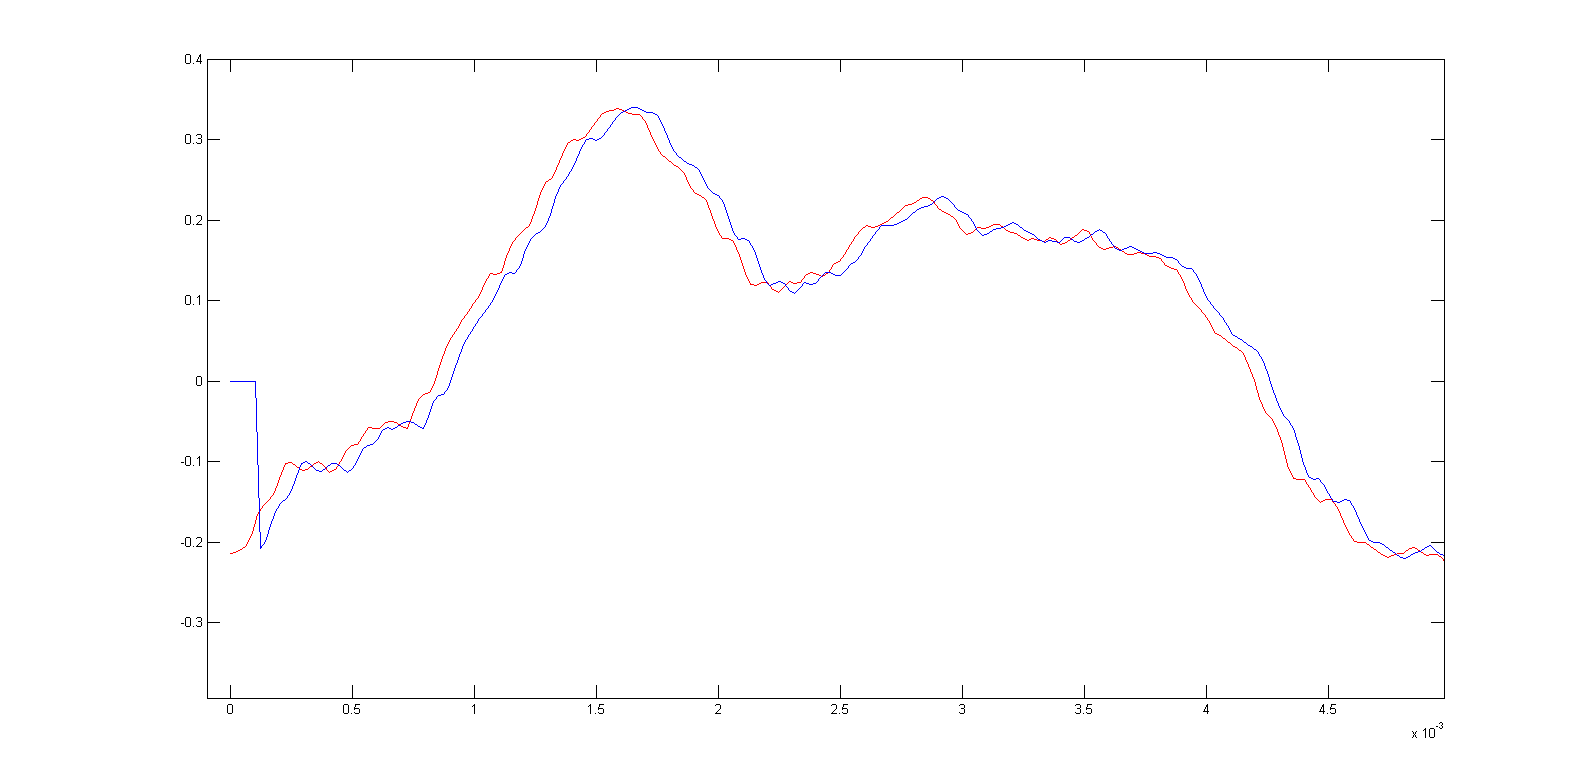
\includegraphics[width=0.7\textwidth]{images/plot1.png}
\caption{Plot of the first part of the original signal (red) and the signal after filtering (blue).}
\label{fig:plot1}
\end{center}
\end{figure}
In figure ~\ref{fig:plot2} we see another plot of the input and output signal. In this plot we have shifted the output signal by -3 samples, and there are dots indicating the samples. We can now see that the output signal has a higher sample frequency than the input signal. 
\begin{figure}
\begin{center}
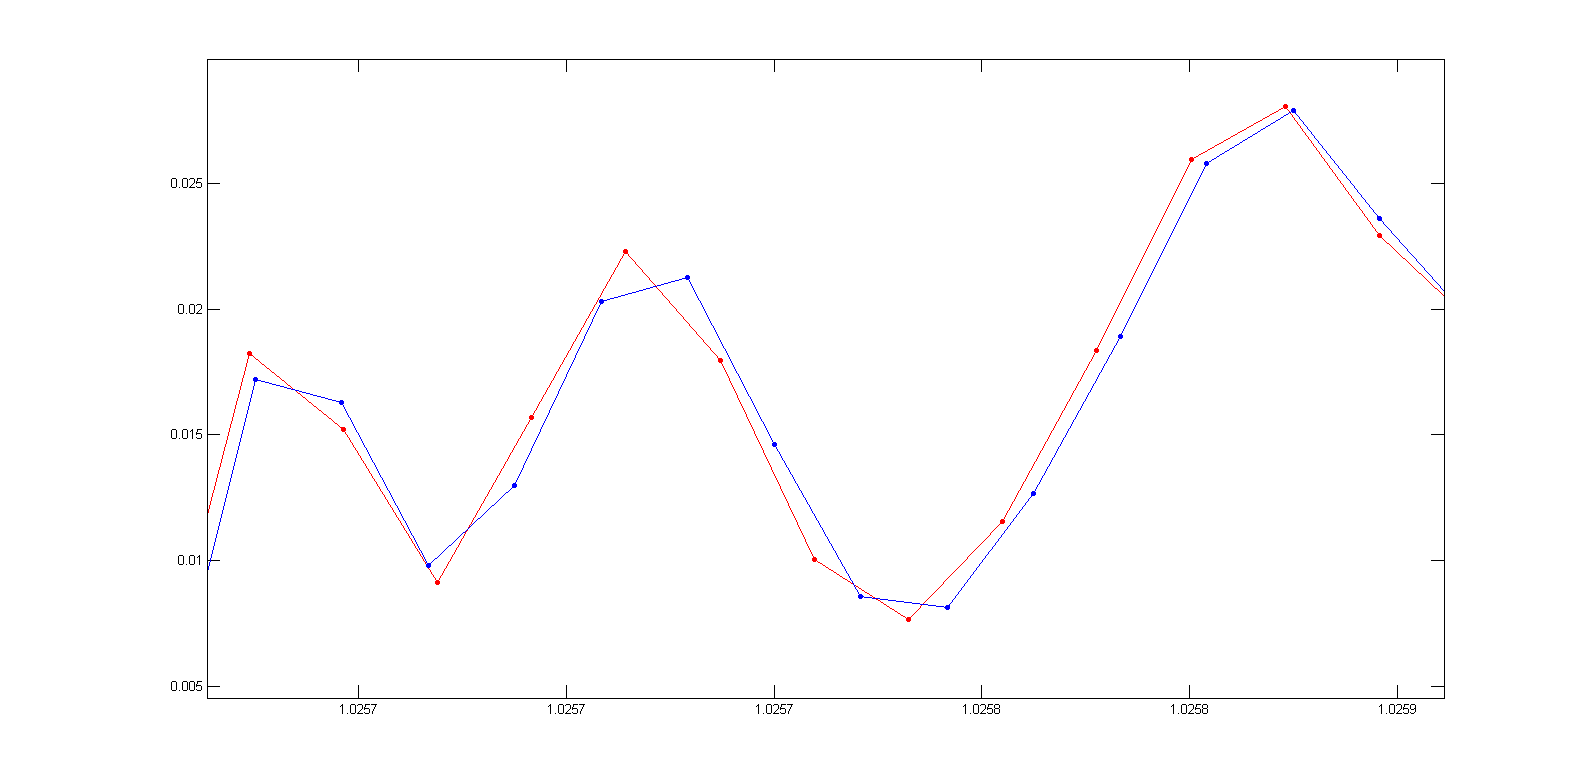
\includegraphics[width=0.7\textwidth]{images/plot2.png}
\caption{Plot of part of the original signal (red) and the signal after filtering (blue) with dots indicating the samples.}
\label{fig:plot2}
\end{center}
\end{figure}
\FloatBarrier
Figure ~\ref{fig:spectrum} shows the signals in the frequency domain. There is only minimal difference between them. The output frequency contains a higher maximum frequency because it has a higher sample rate. 
\begin{figure}
\begin{center}
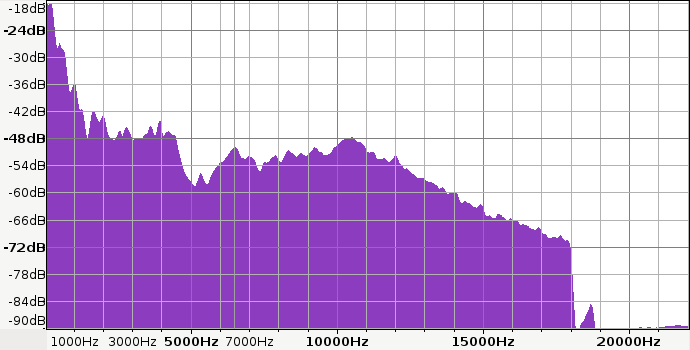
\includegraphics[width=0.7\textwidth]{images/freq1.png}
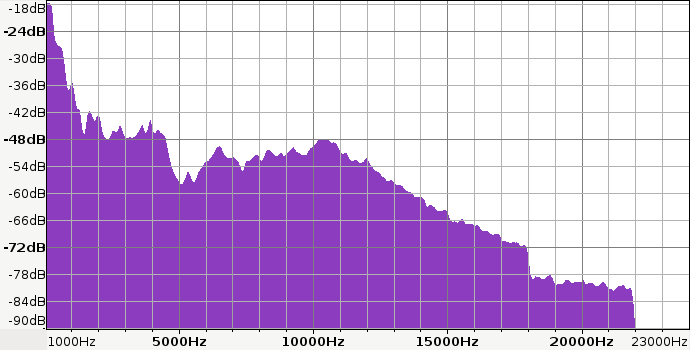
\includegraphics[width=0.7\textwidth]{images/freq2.png}
\caption{Plot in the frequency domain of the original signal (top) and the signal after filtering (bottom).}
\label{fig:spectrum}
\end{center}
\end{figure}
Finally, figure ~\ref{fig:wave} displays some waveforms of the design. For this image we have used $n = 2$. We can see this in the input and output streams, in which \texttt{$<$0000$>$} is interleaved with nonzero values. If we look at \texttt{clk} we can see that we do indeed produce output every clock cycle. We can also see a period in which \texttt{filter\_in\_ack} and \texttt{filter\_req\_ack} are zero, during which input and output remain stable.
\begin{figure}
\begin{center}
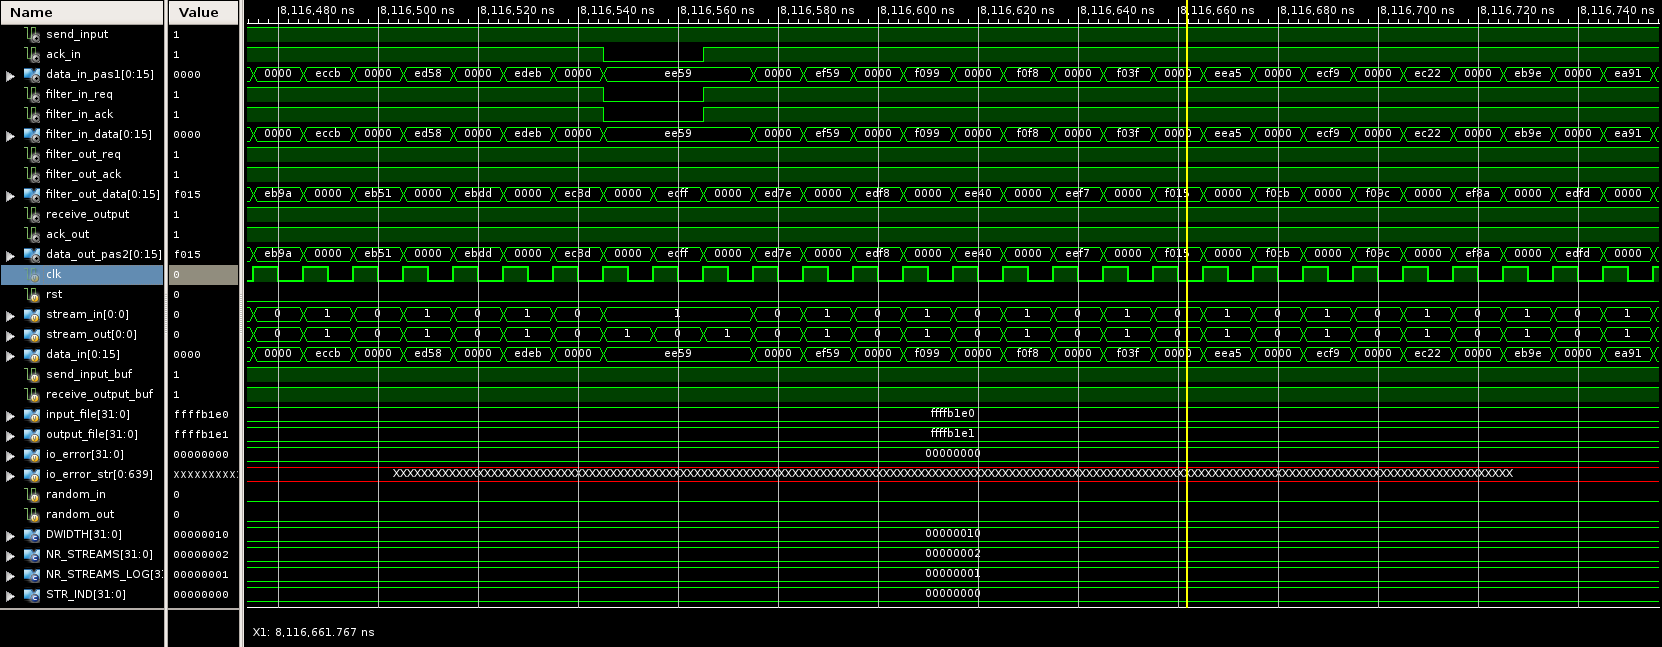
\includegraphics[width=0.7\textwidth]{images/waveforms.png}
\caption{Part of the waveforms of our design.}
\label{fig:wave}
\end{center}
\end{figure}
\FloatBarrier
